\documentclass{article}
\usepackage{tikz}
\usetikzlibrary{shapes.geometric, arrows, positioning}

\tikzstyle{startstop} = [rectangle, rounded corners, minimum width=6cm, minimum height=1cm,text centered, draw=black, fill=green!30]
\tikzstyle{process} = [rectangle, minimum width=6cm, minimum height=1cm, text centered, draw=black, fill=blue!20]
\tikzstyle{decision} = [diamond, aspect=2, text centered, draw=black, fill=orange!30]
\tikzstyle{arrow} = [thick,->,>=stealth]

\begin{document}

\begin{figure}[h!]
\centering
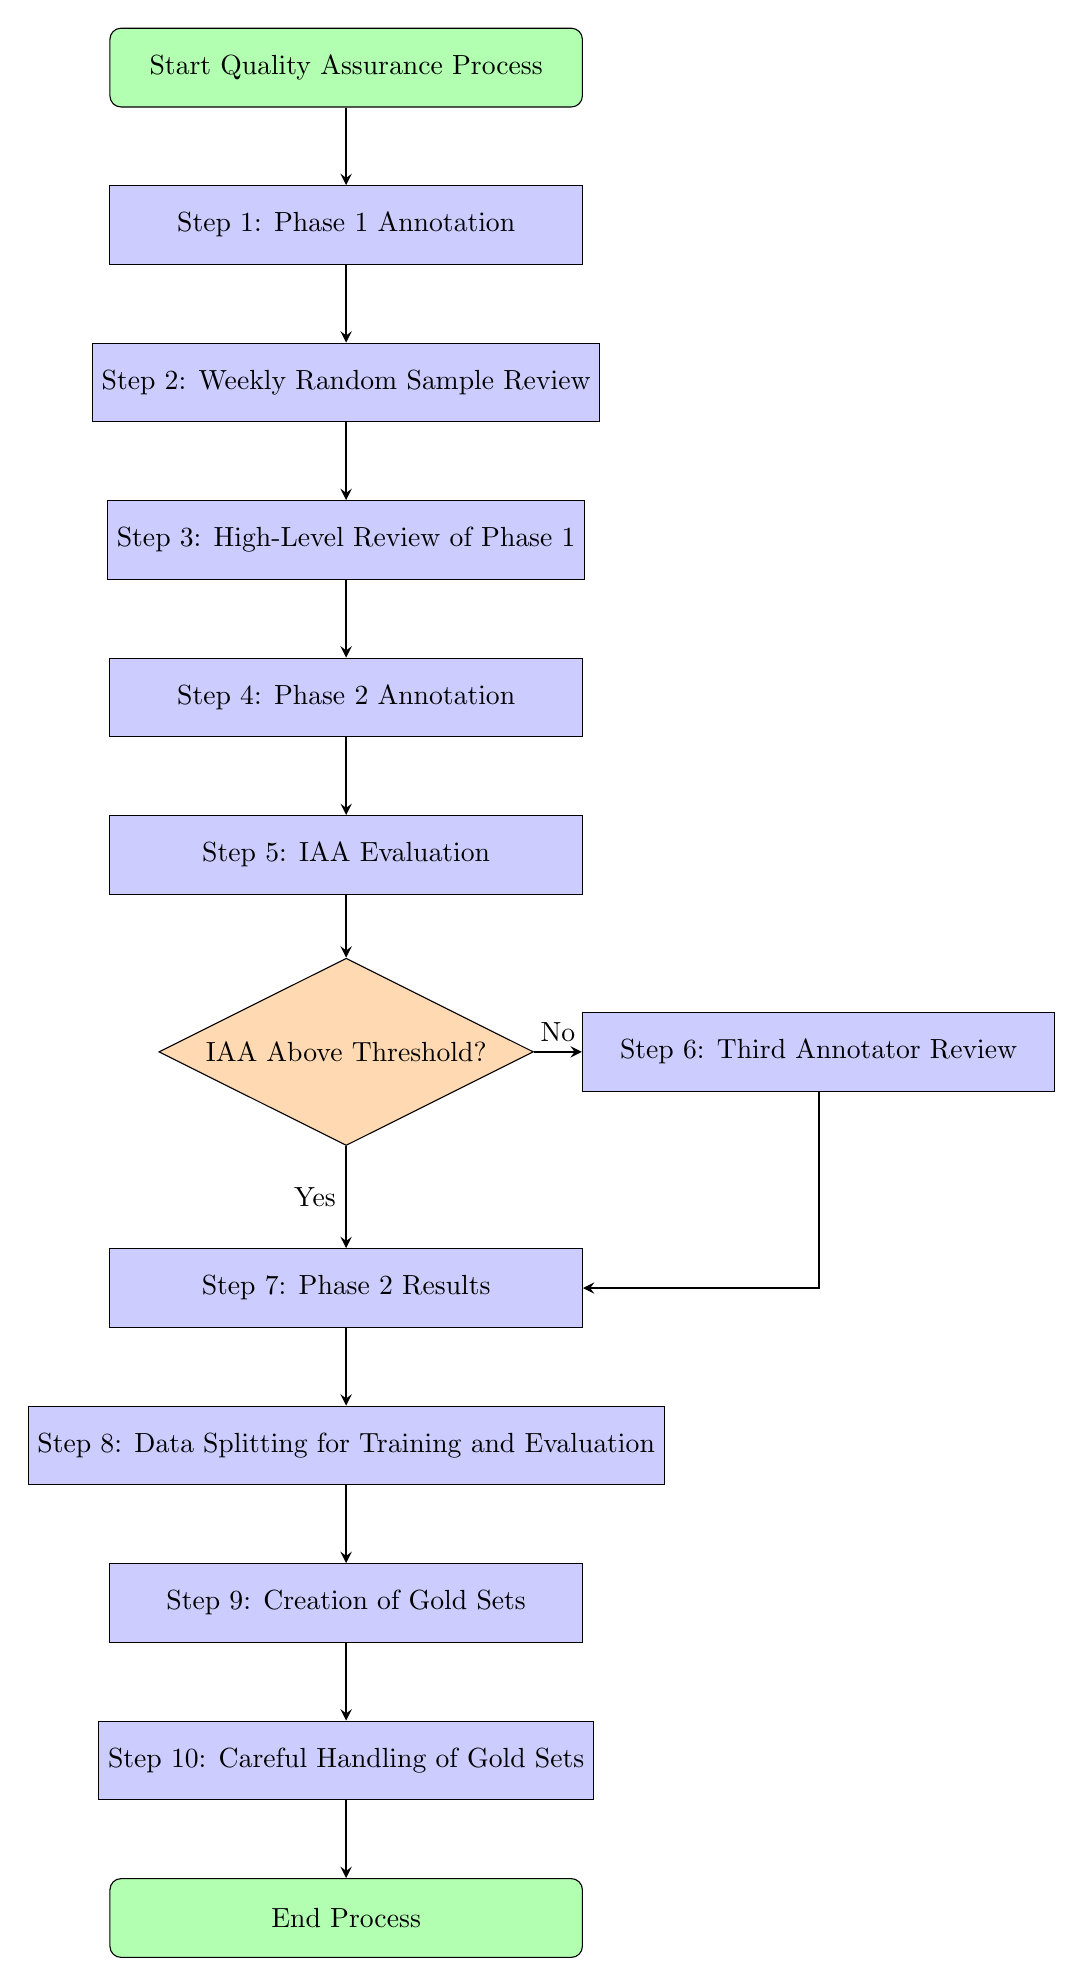
\begin{tikzpicture}[node distance=2cm]

% Nodes
\node (start) [startstop] {Start Quality Assurance Process};

\node (step1) [process, below of=start] {Step 1: Phase 1 Annotation};
\node (step2) [process, below of=step1] {Step 2: Weekly Random Sample Review};
\node (step3) [process, below of=step2] {Step 3: High-Level Review of Phase 1};

\node (step4) [process, below of=step3] {Step 4: Phase 2 Annotation};
\node (step5) [process, below of=step4] {Step 5: IAA Evaluation};
\node (decision1) [decision, below of=step5, yshift=-0.5cm] {IAA Above Threshold?};

\node (step6) [process, right of=decision1, xshift=4cm] {Step 6: Third Annotator Review};

\node (step7) [process, below of=decision1, yshift=-1cm] {Step 7: Phase 2 Results};

\node (step8) [process, below of=step7] {Step 8: Data Splitting for Training and Evaluation};

\node (step9) [process, below of=step8] {Step 9: Creation of Gold Sets};

\node (step10) [process, below of=step9] {Step 10: Careful Handling of Gold Sets};

\node (end) [startstop, below of=step10] {End Process};

% Arrows
\draw [arrow] (start) -- (step1);
\draw [arrow] (step1) -- (step2);
\draw [arrow] (step2) -- (step3);
\draw [arrow] (step3) -- (step4);
\draw [arrow] (step4) -- (step5);
\draw [arrow] (step5) -- (decision1);

\draw [arrow] (decision1) -- node[anchor=east]{Yes} (step7);
\draw [arrow] (decision1) -- node[anchor=south]{No} (step6);
\draw [arrow] (step6) |- (step7);

\draw [arrow] (step7) -- (step8);
\draw [arrow] (step8) -- (step9);
\draw [arrow] (step9) -- (step10);
\draw [arrow] (step10) -- (end);

\end{tikzpicture}
\caption{Flowchart of the Quality Assurance Process}
\end{figure}

\end{document}
